\section{Resultados de Simulação}
\label{sec:resultados}

O sistema foi implementado no Matlab/Simulink utilizando a \textit{toolbox} Specialized Power
Systems, com passo de simulação $T_s/50$ e controle discreto amostrado na frequência de
chaveamento $f_{\sub{sw}}$. O THD foi calculado sobre três ciclos de $i_a$, até a 50ª harmônica.

\subsection{Partida e regime permanente}
Para permitir a pré-carga dos capacitores, o PWM é habilitado em $t=\SI{0,2}{s}$. Após isso,
o controle é totalmente habilitado, podendo-se observar, por meio da Fig.~\ref{fig:tensoes}, que a tensão de barramento ($V_{\sub{dc}}$) atinge
\SI{600}{V} que era a tensão de referência, com um sobressinal de cerca de \SI{20}{V} e as tensões sobre
os capacitores $V_{C1}$ e $V_{C2}$ ficam equilibradas em \SI{300}{V}, com uma ondulação de \SI{\pm 12}{V}. Por fim,
as correntes são senoidais e com cerca de \SI{85,9}{A} de pico.

\begin{figure}[!t]
    \centering
    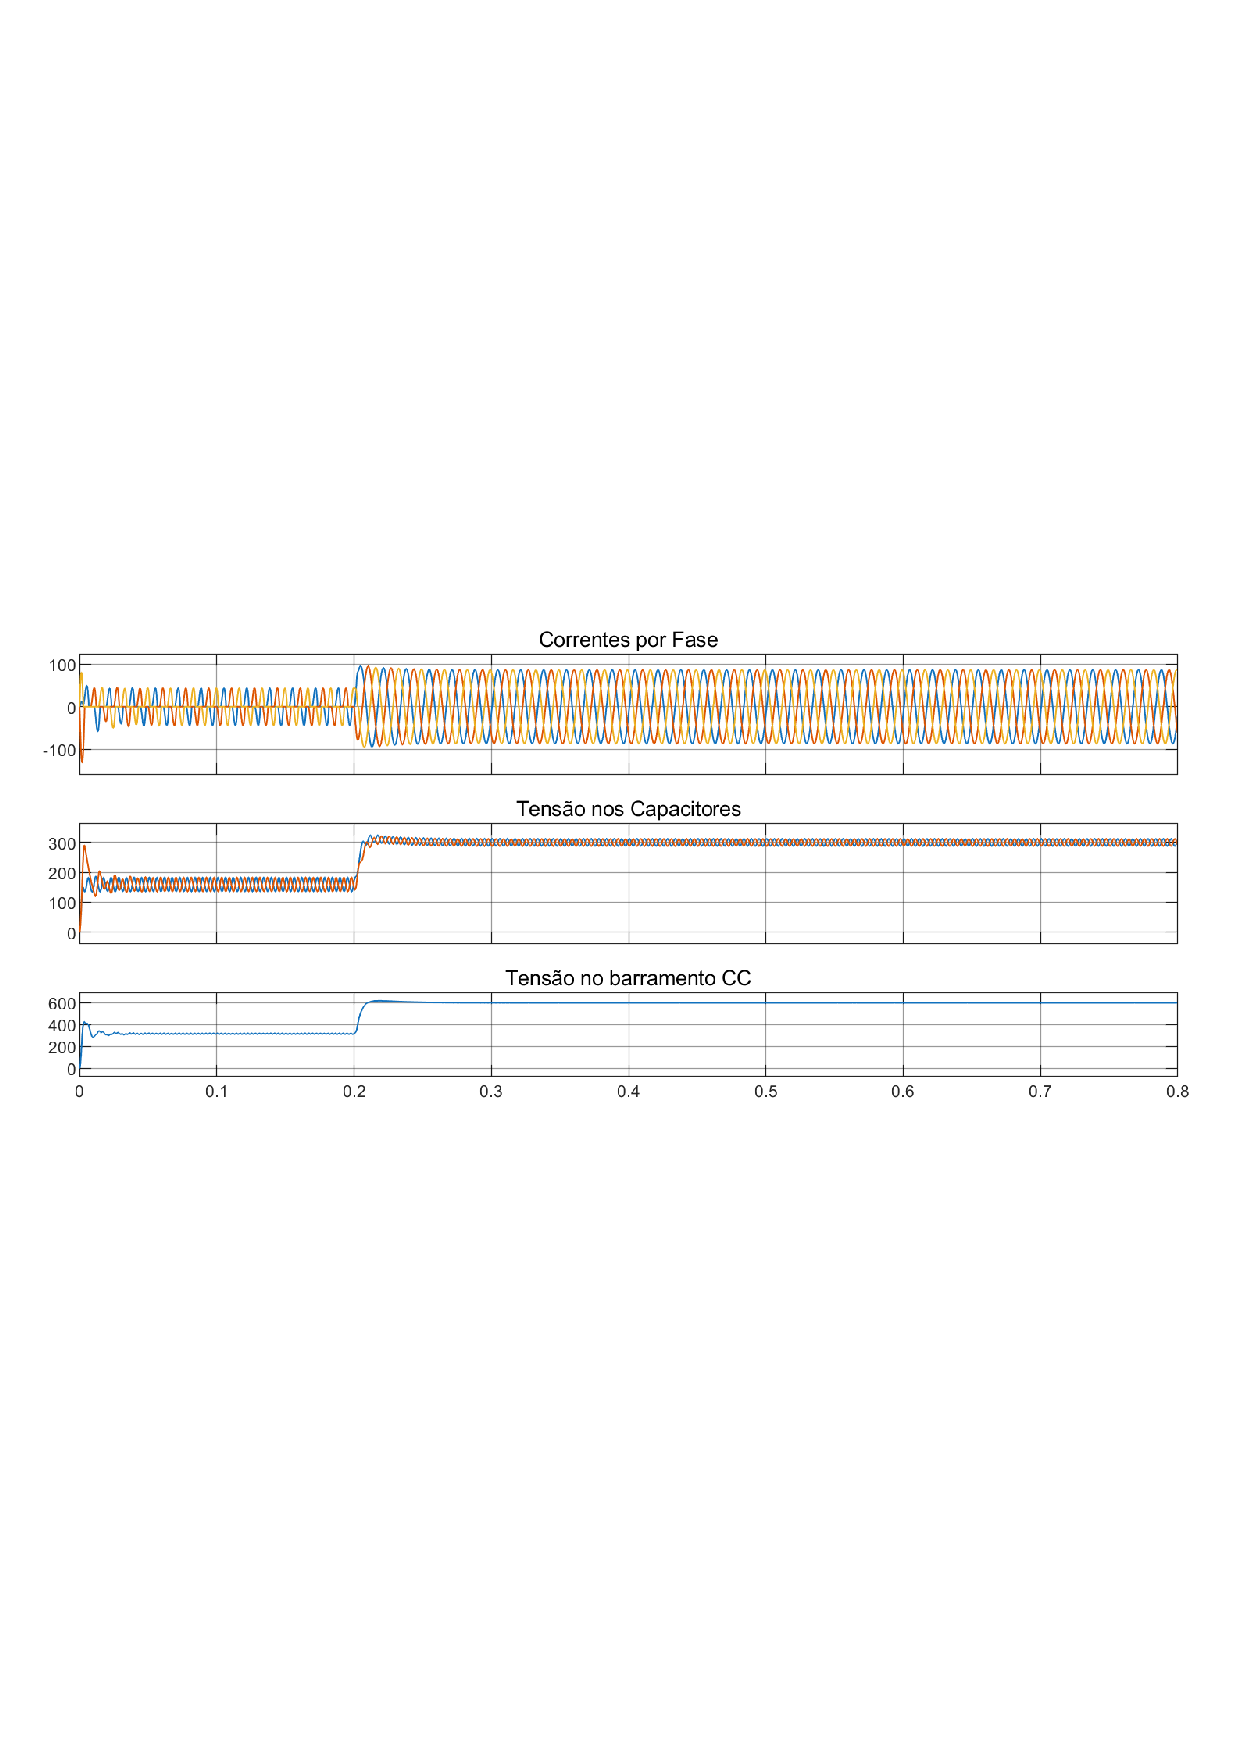
\includegraphics[width=\columnwidth, trim=20 298 20 298, clip]{Tensoes.pdf}
    \caption{Resultados da simulação com limitador ativado.}
    \label{fig:tensoes}
\end{figure}


\subsection{Degraus de Fator de Potência com e sem limitador}

Para verificar se o modelo proposto suportava um PFC, o FP foi variado de 1 para
0,95 indutivo (\SI{0,4}{s}) e depois para 0,95 (\SI{0,6}{s}) capacitivo em carga nominal. Os
resultados são apresentados na Fig.~\ref{fig:potencia} e na Tabela~\ref{tab:res}. Com $\FP^*=1$, o limitador
aplica $\varphi=\ang{7,7}$ e reduz o THD de \SI{7,8}{\percent} para \SI{3,1}{\percent}.

Para o fator de potência em 0,95 indutivo, nota-se que, com e sem limitador, a potência reativa obtida é de \SI{6,8}{kvar} e o FP medido é 0,96, ligeiramente
acima do pedido, pois o reativo é imposto em malha aberta (Tabela~\ref{tab:res}). Nessa situação, é apresentado um THD de \SI{0,3}{\percent}. 

Já para um FP de 0,95 capacitivo, nota-se que, sem limitador, o conversor não é capaz de sintetizar a corrente, uma vez
que conforme discutido na Seção~\ref{sec:modelo}, a tensão necessária teria sinal oposto ao da 
corrente necessária durante cada semiciclo, com isso as razões cíclicas saturam e a corrente se distorce
na passagem por zero
e o THD passa de \SI{20}{\percent}. As harmônicas geradas por essa distorção estão em fase nas três fases e se somam no neutro, elevando
a corrente no neutro e o reativo obtido é menor que o esperado. Com o limitador,
a operação é levada ao limite da janela de operação do retificador ($\varphi \approx \ang{7}$ indutivo), com isso a corrente permanece senoidal, mas o FP medido vai para 0,99 indutivo
conforme é observado nas Figs.~\ref{fig:potencia} e~\ref{fig:potencia2} após \SI{0,6}{s}. A diferença entre o $\FP^*$ e o FP medido é esperada, tendo
em vista que o pedido está fora da região de operação da topologia.

Além disso, pode-se notar também que, em todos os degraus, a potência ativa e a tensão do
barramento CC praticamente não se alteram, o que confirma o desacoplamento previsto anteriormente
em \eqref{eq:decomp}.

\begin{figure}[!t]
    \centering
    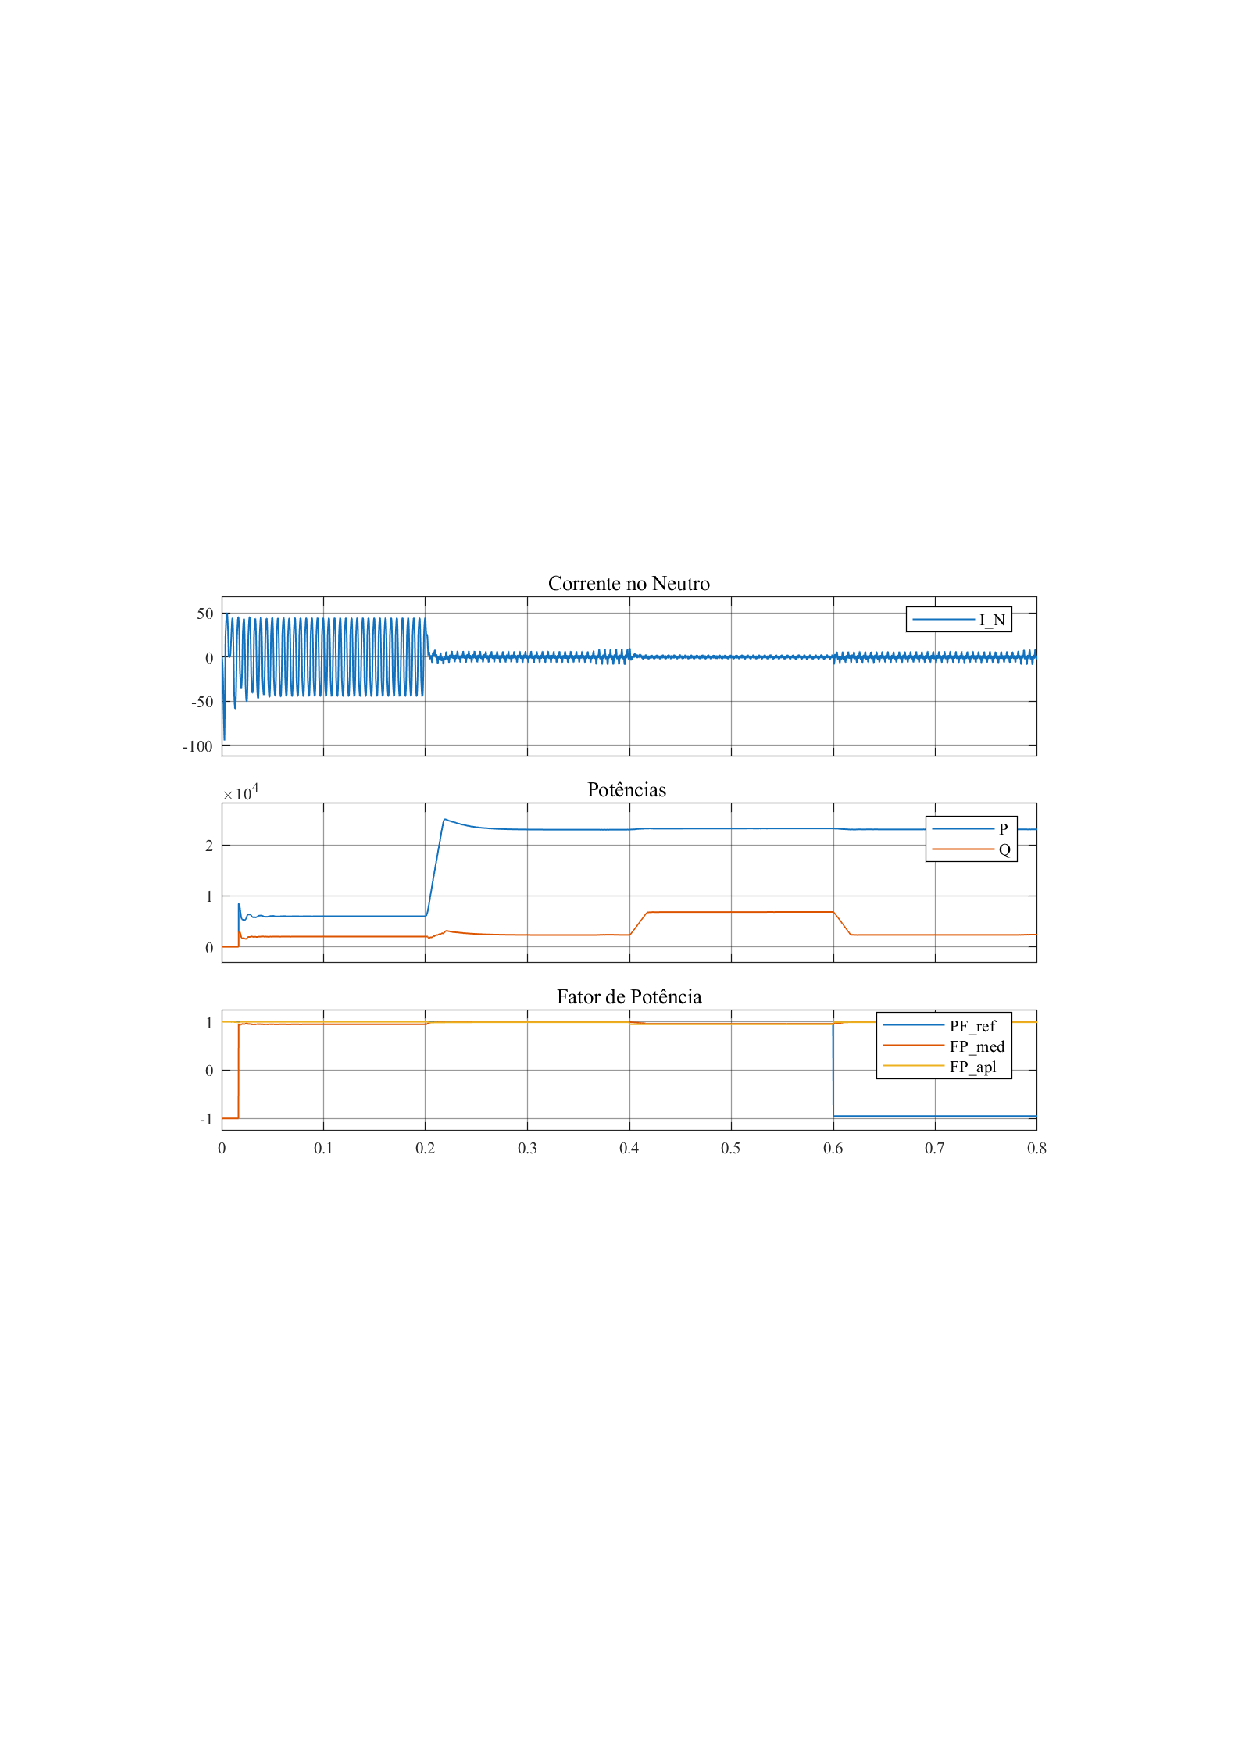
\includegraphics[width=\columnwidth, trim=87 272 87 272, clip]{Potencia2.pdf}
    \caption{Resultados da simulação para corrente no neutro, potências e FP com limitador ativado.}
    \label{fig:potencia}
\end{figure}

\begin{figure}[!t]
    \centering
    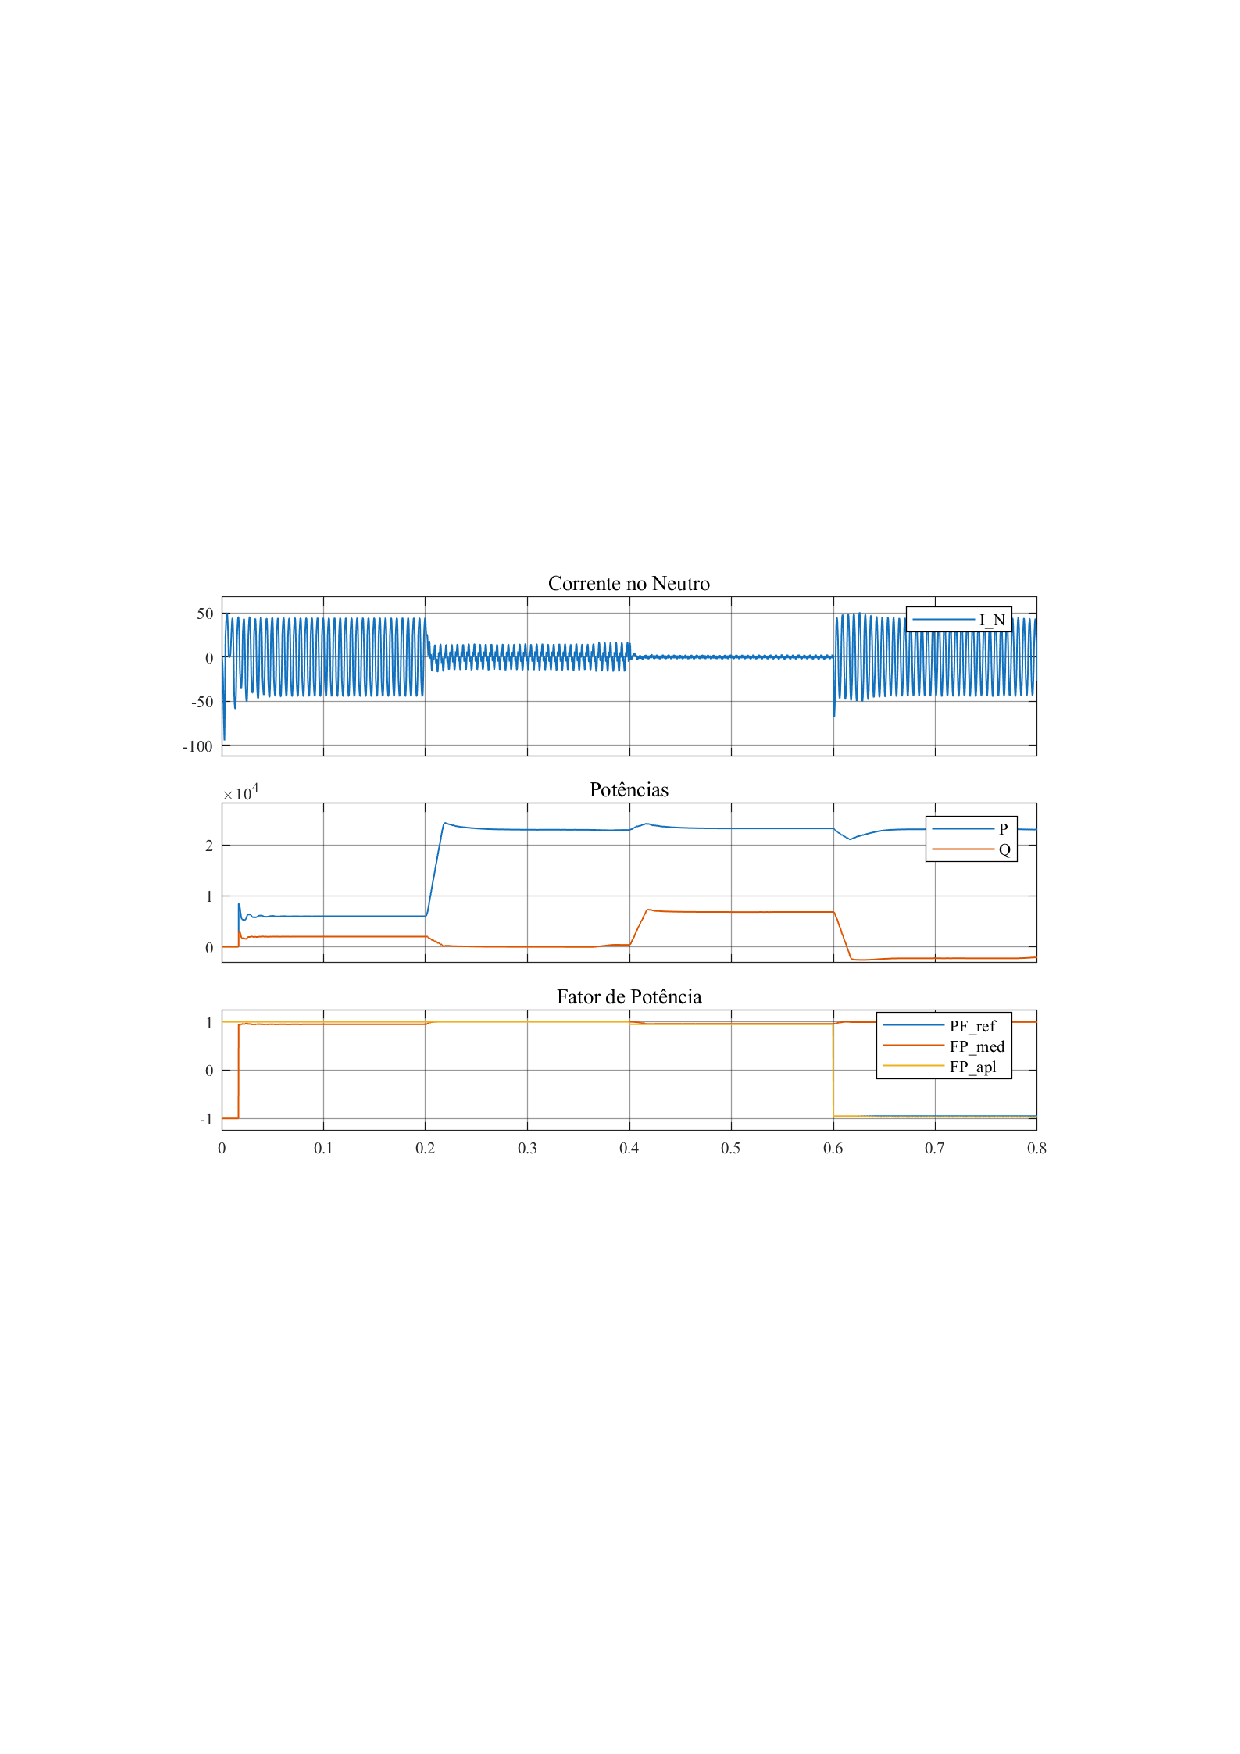
\includegraphics[width=\columnwidth, trim=87 272 87 272, clip]{Potencia2_semlim.pdf}
    \caption{Resultados da simulação para corrente no neutro, potências e FP sem limitador ativado.}
    \label{fig:potencia2}
\end{figure}

\begin{table}[!t]\centering\footnotesize\setlength{\tabcolsep}{3pt}
\caption{Valores de regime nos degraus de FP (carga nominal)}\label{tab:res}
\begin{tabular}{@{}ccccccc@{}}\toprule
\multirow{2}{*}{Intervalo} & \multirow{2}{*}{$\FP^*$} & \multirow{2}{*}{Lim.} & $\varphi$ apl./med. & $Q$ & FP & THD\\
 & & & [\si{\degree}] & [kvar] & medido & [\%]\\\midrule
\multirow{2}{*}{\SIrange{0,3}{0,4}{s}} & \multirow{2}{*}{1} & sim & 7,7/5,8 & 2,3 & 0,995 ind. & 3,1\\
 & & não & 0,0/0,5 & 0,2 & 1,000 & 7,8\\\midrule
\multirow{2}{*}{\SIrange{0,4}{0,6}{s}} & \multirow{2}{*}{0,95 ind.} & sim & 18,2/16,4 & 6,8 & 0,959 ind. & 0,3\\
 & & não & 18,2/16,4 & 6,8 & 0,959 ind. & 0,3\\\midrule
\multirow{2}{*}{\SIrange{0,6}{0,8}{s}} & \multirow{2}{*}{0,95 cap.} & sim & 7,7/5,8 & 2,3 & 0,995 ind. & 2,7\\
 & & não & $-14{,}5$/$-5{,}5$ & $-2{,}2$ & 0,995 cap. & 20,1\\\bottomrule
\end{tabular}\end{table}

\subsection{Operação com tensões distorcidas}

Para avaliar a operação com rede distorcida, foi adicionada à fonte, a partir de $t=\SI{0,3}{s}$, uma quinta harmônica de sequência negativa com \SI{5}{\percent} e
uma sétima harmônica de sequência positiva com \SI{3}{\percent} da fundamental, mantendo os intervalos de fator de potência como descritos para o caso anterior. Foram
simulados dois casos, um com as duas harmônicas na fase \ang{0} e outro com as duas harmônicas na fase \ang{180}. Em ambos os casos, os ângulos medidos e
as potências ativa e reativa permaneceram iguais às apresentadas na Tabela~\ref{tab:res}. Essa manutenção de resultados comprova o funcionamento
do rastreamento de ângulo do PLL.

No intervalo de $\FP^*=0{,}95$ indutivo, sem a atuação do limitador, o THD passou de \SI{0,3}{\percent} para \SI{1,3}{\percent} para as harmônicas em \ang{0} e para \SI{1,2}{\percent} para as harmônicas
em \ang{180}. Nos intervalos próximos à borda da janela de fator de potência estabelecida, notou-se que, para as harmônicas em \ang{0}, o THD caiu de \SI{3,1}{\percent} para \SI{1,5}{\percent} para $\FP^*=1$
e, na faixa capacitiva, foi de \SI{2,7}{\percent} para \SI{1,3}{\percent}; já com \ang{180}, os valores subiram para \SI{5,9}{\percent} e \SI{5,5}{\percent}, respectivamente. Isso ocorre porque as harmônicas
alteram a forma da tensão próxima à passagem por zero e, conforme a fase, encurtam ou alongam o trecho de sinais opostos na borda da janela. Sem a utilização do limitador,
para \ang{0}, o THD foi de \SI{6,2}{\percent} com $\FP^*=1$ e de \SI{19,5}{\percent} no pedido de fator de potência capacitivo. Dessa forma, percebeu-se que a vantagem do limitador
é mantida com a rede distorcida, mas, para o caso de distorções harmônicas na rede, a janela $\Delta$ escolhida para a rede senoidal não garante THD abaixo de
\SI{5}{\percent}.

